\documentclass[border=3pt,tikz]{standalone}
\usepackage{bm,amsmath}
\usetikzlibrary{patterns,decorations.pathmorphing,decorations.text}
\usetikzlibrary{arrows.meta}
\usetikzlibrary{calc}


\begin{document}

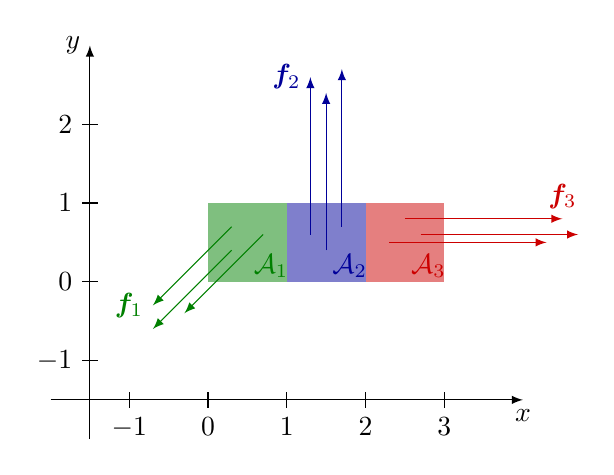
\begin{tikzpicture}[scale=1.0]


  \fill[green!50!black,opacity=0.5] (0,0) rectangle (1,1);
  \fill[blue!60!black,opacity=0.5] (1,0) rectangle (2,1);
  \fill[red!80!black,opacity=0.5] (2,0) rectangle (3,1);

  \draw[-latex,green!50!black] (0.7,0.6) -- ++(-1,-1);
  \draw[-latex,green!50!black] (0.3,0.4) -- ++(-1,-1);
  \draw[-latex,green!50!black] (0.3,0.7) -- ++(-1,-1) node[left,pos=1] {$\bm{f}_1$};

  \draw[-latex,blue!60!black] (1.7,0.7) -- ++(0,2);
  \draw[-latex,blue!60!black] (1.5,0.4) -- ++(0,2);
  \draw[-latex,blue!60!black] (1.3,0.6) -- ++(0,2) node[left,pos=1] {$\bm{f}_2$};

  \draw[-latex,red!80!black] (2.7,0.6) -- ++(2,0);
  \draw[-latex,red!80!black] (2.5,0.8) -- ++(2,0) node[above,pos=1] {$\bm{f}_3$};
  \draw[-latex,red!80!black] (2.3,0.5) -- ++(2,0);

  \node[anchor=center,green!50!black] at (0.8, 0.2) {$\mathcal{A}_1$};
  \node[anchor=center,blue!60!black] at (1.8, 0.2) {$\mathcal{A}_2$};
  \node[anchor=center,red!80!black] at (2.8, 0.2) {$\mathcal{A}_3$};

  \draw[-latex,black] (-2,-1.5)--++(6,0) node[below,pos=1] {$x$};
  \draw[-latex,black] (-1.5,-2)--++(0,5) node[left,pos=1] {$y$};
  \draw (0,-1.4)--++(0,-0.2) node[below, pos=1] {$0$};
  \draw (-1.4,0)--++(-0.2,0) node[left, pos=1] {$0$};

  \draw (1,-1.4)--++(0,-0.2) node[below, pos=1] {$1$};
  \draw (-1.4,1)--++(-0.2,0) node[left, pos=1] {$1$};

  \draw (2,-1.4)--++(0,-0.2) node[below, pos=1] {$2$};
  \draw (-1.4,2)--++(-0.2,0) node[left, pos=1] {$2$};

  \draw (3,-1.4)--++(0,-0.2) node[below, pos=1] {$3$};

  \draw (-1,-1.4)--++(0,-0.2) node[below, pos=1] {$-1$};
  \draw (-1.4,-1)--++(-0.2,0) node[left, pos=1] {$-1$};


\end{tikzpicture}

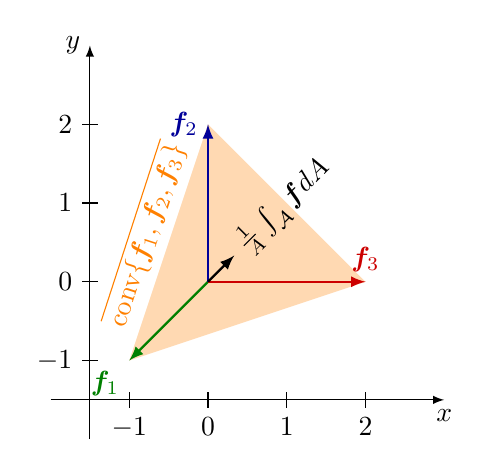
\begin{tikzpicture}[scale=1.0]

  \coordinate (O) at (0,0);
  \coordinate (f1) at (-1,-1);
  \coordinate (f2) at (0,2);
  \coordinate (f3) at (2,0);
  \coordinate (fave) at (0.3333,0.3333);

  \fill[orange,opacity=0.3] (f1)--(f2)--(f3)--cycle;
  \node[orange,anchor=center,rotate=72] at (-0.8,0.6) {$\overline{\text{conv}\{\bm{f}_1,\bm{f}_2,\bm{f}_3\}}$};

  \draw[-latex,thick,green!50!black] (O)--(f1) node[below left,pos=1] {$\bm{f}_1$};
  \draw[-latex,thick,blue!60!black] (O)--(f2) node[left,pos=1] {$\bm{f}_2$};
  \draw[-latex,thick,red!80!black] (O)--(f3) node[above,pos=1] {$\bm{f}_3$};
  \draw[-latex,black,thick] (O)--(fave) node[right,pos=1,rotate=45] {$\frac{1}{A}\int_\mathcal{A} \bm{f} dA$};

  \draw[-latex,black] (-2,-1.5)--++(5,0) node[below,pos=1] {$x$};
  \draw[-latex,black] (-1.5,-2)--++(0,5) node[left,pos=1] {$y$};
  \draw (0,-1.4)--++(0,-0.2) node[below, pos=1] {$0$};
  \draw (-1.4,0)--++(-0.2,0) node[left, pos=1] {$0$};

  \draw (1,-1.4)--++(0,-0.2) node[below, pos=1] {$1$};
  \draw (-1.4,1)--++(-0.2,0) node[left, pos=1] {$1$};

  \draw (2,-1.4)--++(0,-0.2) node[below, pos=1] {$2$};
  \draw (-1.4,2)--++(-0.2,0) node[left, pos=1] {$2$};

  \draw (-1,-1.4)--++(0,-0.2) node[below, pos=1] {$-1$};
  \draw (-1.4,-1)--++(-0.2,0) node[left, pos=1] {$-1$};

\end{tikzpicture}

\end{document}
  
